\subsection{Data Object Storage}
\label{apx:data-object-storage}

In the section ~\ref{sec:architecture} we supposed that all student's solutions,
papers, assignments and so on are stored locally on the educator's servers. But
it should be possible to introduce the new entity called "Data Object Storage"
to our model(fig. ~\ref{fig:entities}). This entity should support an encrypted
distributed access to all student's works. The main purposes of the data object
storage are:

\begin{itemize}
\item to make publications more accessible for everyone.
\item to get rid educators of the need to store a lot of information locally without loss of security.
\end{itemize}

\begin{figure}[ht]
\centering
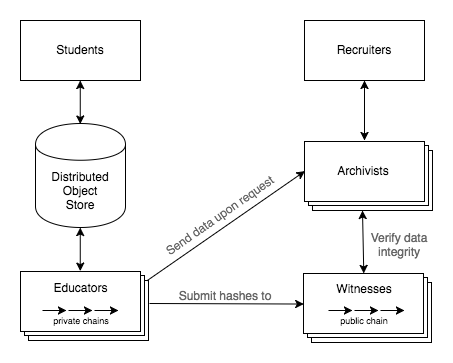
\includegraphics[width=0.7\textwidth]{entities}
\caption{Entities of the Disciplina platform including distributed object storage}
\label{fig:entities}
\end{figure}
